\documentclass[12pt]{article}
\usepackage[english]{babel}
\usepackage[utf8x]{inputenc}
\usepackage{amsmath}
\usepackage{graphicx}
\usepackage[colorinlistoftodos]{todonotes}

\begin{document}

\begin{titlepage}

\newcommand{\HRule}{\rule{\linewidth}{0.5mm}} % Defines a new command for the horizontal lines, change thickness here

\center % Center everything on the page

\textsc{\LARGE University of Rochester}\\[1.5cm] % Name of your university/college
\textsc{\Large CSC 242}\\[0.5cm] % Major heading such as course name
\textsc{\large Artificial Intelligence}\\[0.5cm] % Minor heading such as course title

\HRule \\[0.4cm]
{ \huge \bfseries Neural Networks for Learning}\\[0.4cm] % Title of your document
\HRule \\[1.5cm]

\Large \emph{Author:}\\
Edan \textsc{Meyer}\\[2cm] % Your name

{\large April 27, 2017}\\[2cm] % Date, change the \today to a set date if you want to be precise


\includegraphics[width=3.5cm,height=3.5cm,keepaspectratio]{img/logo.png}\\[1cm] % Include a department/university logo - this will require the graphicx package

\vfill % Fill the rest of the page with whitespace

\end{titlepage}

\section{Introduction}

In my write up, I cover the trial and results of testing the neural network I built in Python over the
Iris Plant training data. I first explain how the neural network works and processes the testing data, then move on to evaluate the accuracy of the system and how to maximize its efficiency.

\section{Training Data}
I use the Iris Plants Database to train my network. The database consists of a total of 150 samples, each of which contains four attributes and one output. The four attributes are
attributes of the Iris flower, and are as follows:
\begin{itemize}
\item Sepal length in cm
\item Sepal width in cm
\item Petal length in cm
\item Petal width in cm
\end{itemize}
The output of the dataset is the type of Iris flower the plant is. There are three possibilities:
\begin{itemize}
\item Iris Setosa
\item Iris Versicolour
\item Iris Virginica
\end{itemize}
Thus, the goal of the nerual network is to, given the value of the four attributes of the the flower, predict what type of Iris it is.
Do keep in mind, however, that even though this is the data set used for exploring the use of the neural network, the neural network has a
dynamic amount of input, hidden, and output nodes, so it can work with a large variety of datasets.

\section{Using the Network}
\subsection{Forward Propogation}

The network begins by establishing two layers of weights that are assigned random values
between 0 and 0.5 to start with. To get the values of the hidden layers the input values are
multiplied by the first set of weights and added up at each individual hidden node. Each value at
the hidden nodes is then put through the activation function (which will be discussed later).The
same is then done to get the values at the output nodes.

\subsection{Fast Calculations}

Rather than using a typical summation and having a for loop that multiplies every individual node by
the individual weights, the values of all sets of nodes and all sets of weights are stored in matrices
that I use numpy to evaluate. Using matrices provides many benefits for which reason they are
commonly used in nearly every popular neural network implementation. They make code much
cleaner because they reduce calculations that would take several lines to single lines containing
just a few characters. Additionally, matrix multiplication, unlike many other types of math, can be
pushed to a GPU, which speeds up the process of training and prediction by a factor of usually 10
or more. I did not include the GPU in this project because more libraries and overhead beyond the
scope of the project would have been required, but the network is setup so that GPU math could
be implemented while keeping the same basic structure.

\subsection{Activation Function}

The activation function I used was a sigmoid logistic function:
$$\dfrac{1}{1+e^{-x}}$$
While the iris result value is either 0, 1, or 2 depending on the type of flower, I don’t use a hard
cutoff, and instead, round the result at the end due to the many benefits of using the sigmoid
function. When finding how to change the weights, it is necessary to calculate the derivative of the
activation function if you are making use of gradient descent (which I did). Luckily, the derivative of
the sigmoid function is very simple and easy to compute:
$$where f(x) = \dfrac{1}{1+e^{-x}}, f’(x) = f(x)(1 - f(x))$$
Not only is the function easy to derive, but when working with real world data, a sigmoid function
like the one I used works much better on average when taking into account any uncertainty in the
data, or attributes that may not be perfectly difinitive, which is often the case in the real world.

\subsection{Loss Calculation}

$L_2$ loss is used to calculate loss. I make use of it because it is parabolic which means it has
one global minimum, which makes it very easy to minimize. In addition, it is easy to calculate. The
calculation of  $L_2$ loss is as follows:
$$L_2 = (Y_{actual} - Y_{predicted})^2$$
The value of the weights it changed by the negative derivative of the $L_2$ function multiplied by
the loss itself and alpha, a constant. Where $g$ is the activation function, the derivative of the $L_2$ function is:
$$g(out_{i-1}) \cdot -(Y - g(out_{i})) \cdot g’(out_{i})$$
where the first product on the left works like matrix multiplication and the one after works like
vector multiplication.

\subsection{Learning Rate}

Earlier it was mentioned that $\alpha$ was a constant multiplied by the weight change. $\alpha$ is the
learning rate that decides how fast the weights are changed. With a smaller alpha, there is a
greater chance that the loss will converge, but slower changing rates means that more calculation
time is necessary. A higher learning rate means that weights will change faster and less
calculation time is needed, but it is possible that the loss won't converge at a low value and will
skip over the lowest point. I have it configured to run a total of 500 loops on 135 data points, for a
total of 67,500 training loops. After testing different values, even though learning rates are typically
less than one, I found that the value of one for alpha worked very well for the data. The graph below shows a
comparison between the number of loops over all the data and the loss, with a learning rate of
one.
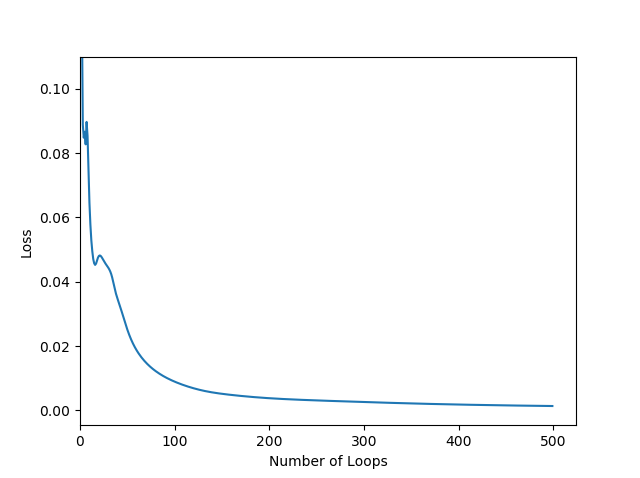
\includegraphics{img/trainvsloss.png}
As seen, the loss rate starts to converge and flatten out between 200 and 300 loops, which only
takes about three to four seconds!

\subsection{Testing}

I randomized all the data before saving it, so there is no selected order. When training and testing,
I separate my data into two tests for training and testing. Training uses 90\% of the data while
testing uses the 10\% that is left. There are an overall 150 data points, which leaves 15 tests. After
training, the the net has higher than 93\% accuracy in predicting. While it’s not perfect, with only 15
points to test on, it is hard to tell exactly how accurate the predictions are. There is a chance that it
could be much closer to 100\% accurate. And even 93\% is fairly good.

\end{document}
